\documentclass[11pt,a4paper]{article}

% ── Core packages — matching invisible_bridges.tex ───────────────────────────
\usepackage[utf8]{inputenc}
\usepackage[T1]{fontenc}
\usepackage{microtype}
\usepackage[margin=1in]{geometry}
\usepackage{amsmath,amssymb,amsfonts,amsthm}
\usepackage{graphicx}
\graphicspath{{figures/}}
\usepackage{booktabs}
\usepackage{multirow}
\usepackage{subcaption}
\usepackage{float}
\usepackage{xcolor}
\usepackage{algorithm}
\usepackage{algpseudocode}
\usepackage[round,sort]{natbib}
\usepackage{hyperref}
\usepackage{url}
\usepackage{enumitem}
\usepackage{tabularx}
\usepackage{array}
\usepackage{setspace}

% ── Hyperref configuration ────────────────────────────────────────────────────
\hypersetup{
    colorlinks = true,
    linkcolor  = blue!70!black,
    citecolor  = green!50!black,
    urlcolor   = blue!80!black,
    pdftitle   = {Shared Perturbation Geometry in Transformer Representations},
    pdfauthor  = {Amit Kumar}
}

% ── Custom maths commands ─────────────────────────────────────────────────────
\newcommand{\R}{\mathbb{R}}
\newcommand{\E}{\mathbb{E}}
\newcommand{\hb}{\bar{h}}
\newcommand{\pr}{\text{PR}}

\theoremstyle{definition}
\newtheorem{definition}{Definition}[section]
\theoremstyle{plain}
\newtheorem{proposition}{Proposition}[section]

% ── Title block ───────────────────────────────────────────────────────────────
\title{%
    \LARGE\textbf{Shared Perturbation Geometry in Transformer Representations}%
}

\author{%
    Amit Kumar\\[2pt]
    \small\textit{Independent Researcher}\\
    \small\texttt{[contact email]}%
}

\date{\today}

% ═════════════════════════════════════════════════════════════════════════════
\begin{document}

\maketitle
\thispagestyle{empty}

% ── Abstract ─────────────────────────────────────────────────────────────────
\begin{abstract}
\noindent
We investigate how representational perturbations propagate downstream in transformer language models. Rather than mapping discrete, graph-like routing circuits, we characterize the global propagation of representation shifts empirically. By performing systematic ablations across every layer in four distinct model families (GPT-2, Pythia, Qwen, and Gemma), we show that downstream perturbations are concentrated within a shared, low-dimensional subspace. Every layer projects downstream perturbations along nearly identical directions, with the first right singular vector ($v_1$) exhibiting an average off-diagonal cosine similarity of 0.935--0.976 across all layer pairs. Within this shared geometry, the effective routing dimensionality remains low (observed trace-based participation ratio $\approx 1.1$--$3.2$ vs. shuffled matrix baseline $\approx 2.7$--$11.5$), and the first singular component explains over 90\% of downstream variance. Causally critical ``bridge'' heads do not drive perturbations in distinct directions; instead, they act as specialized amplitude injectors, driving substantially larger perturbations along the same globally shared subspace. These results suggest that representation routing in transformers is consistent with a shared low-dimensional routing geometry that complements localized circuit-level computation.
\end{abstract}

\newpage
\setcounter{page}{1}
\tableofcontents
\vspace{2em}

% ═════════════════════════════════════════════════════════════════════════════
\section{Introduction}
\label{sec:intro}

A central goal of mechanistic interpretability is to understand how information flows through transformer language models. Typical approaches frame this flow in the language of discrete circuits—subgraphs of attention heads and MLP layers that perform specialized sub-computations, such as induction or indirect object identification. Under this view, representation routing is highly localized, with distinct heads communicating via independent pathways.

In this work, we propose a different perspective. Rather than assuming discrete routing pathways, we empirically map the downstream hidden-state perturbations caused by ablating individual attention heads. We scale this targeted ablation mapping to \emph{every layer} across four decoder-only transformer families: GPT-2, EleutherAI Pythia, Alibaba Qwen, and Google Gemma. 

Our empirical results reveal a striking geometric constraint: downstream perturbations do not disperse isotropically or along head-specific paths. Instead, they collapse into a \textbf{globally aligned, low-dimensional routing geometry}. Every layer projects its downstream representation shifts along virtually the same dominant direction. The first right singular vector ($v_1$) of the downstream influence matrix exhibits an average pairwise cosine similarity of over 0.97 in GPT-2 and over 0.93 in Qwen, indicating that the primary perturbation direction is nearly invariant across layers.

Within this shared highway, we find that the intrinsic dimensionality of the routing subspace is extremely low across all models (Participation Ratio $\approx 1.1$--$3.2$), while the dominant singular component explains over 90\% of all downstream variance. Finally, we characterize the role of causally critical ``bridge'' heads within this framework. We show that bridge heads are not outliers in the direction of their downstream influence; instead, they are \textbf{localized amplitude injectors} that drive disproportionately larger perturbations along the same shared routing subspace.

\paragraph{Why this paper?}
This paper is driven by a single question: \emph{Do downstream representation
perturbations in a transformer collapse onto a shared, low-dimensional
routing manifold?} Prior mechanistic-interpretability work frames routing
as discrete, localized circuits; we instead ask whether the global
propagation of representation shifts is geometrically constrained. By
mapping ablations across every layer of four model families and analyzing
the resulting influence matrices via singular-value decomposition, we find
that perturbations from different source layers align to a nearly invariant
dominant direction while remaining extremely low-dimensional---suggesting
that routing is organized around a conserved subspace that complements,
rather than contradicts, localized circuit computation.

% ═════════════════════════════════════════════════════════════════════════════
\section{Methods: Mapping Downstream Representation Geometry}
\label{sec:methods}

To characterize representation routing without imposing structural graph assumptions, we define a set of empirical metrics to measure the magnitude, dimensionality, and alignment of downstream perturbations.

\subsection{Downstream Pairwise Influence}
Let $M$ be a transformer with $L$ layers and $H$ attention heads per layer, yielding $N = L \times H$ total heads. Let $h_v(x) \in \mathbb{R}^{T \times d_h}$ denote the activation representation of downstream head $v$ (at layer $l_v > l_u$) for an input sequence $x$ of length $T$, where $d_h$ is the head dimension. Let $h_v^{(\backslash u)}(x)$ denote the representation of head $v$ when source head $u$ (at layer $l_u$) is ablated. 

We define the downstream representation influence $I(u, v)$ as the average fractional change in the L2 norm of the activations across sequence positions (reported as fractions, where e.g., $0.21$ corresponds to a $21\%$ change):
\begin{equation}
    I(u, v) \;=\; \E_{x \sim \mathcal{P}} \left[ \frac{1}{T} \sum_{t=1}^T \frac{\|h_{v, t}(x) - h_{v, t}^{(\backslash u)}(x)\|_2}{\|h_{v, t}(x)\|_2 + \epsilon} \right]
    \label{eq:influence}
\end{equation}
where $\epsilon = 10^{-8}$ is a numerical stabilizer. For any source head $u$, this yields an influence vector $I_u \in \mathbb{R}^{N_{down}}$, where $N_{down}$ is the number of target heads downstream from layer $l_u$. Collecting these vectors across all source heads in a given layer $l$ produces the layer-wise influence matrix $I_l \in \mathbb{R}^{H \times N_{down}}$.

\subsection{Frobenius Routing Norm}
To measure the total volume of downstream perturbation injected by a layer $l$, we define the Frobenius Routing Norm:
\begin{equation}
    E_{F}(l) \;=\; \|I_l\|_F \;=\; \sqrt{\sum_{u \in \text{layer } l} \sum_{v > l} I(u, v)^2}
    \label{eq:frobenius}
\end{equation}
This metric captures the localized routing intensity, highlighting layers that act as primary perturbation amplifiers.

\subsection{Effective Dimensionality (Singular-Value Participation Ratio)}
To quantify the sparsity and dimensionality of the downstream influence, we compute the Singular Value Decomposition (SVD) of the influence matrix $I_l$. Let $\{s_i\}$ be the singular values of $I_l$. The effective dimensionality of the perturbation space is measured via a trace-based, singular-value participation ratio ($\pr$):
\begin{equation}
    \pr(l) \;=\; \frac{\left( \sum_{i} s_i \right)^2}{\sum_{i} s_i^2}
    \label{eq:pr}
\end{equation}
We define the participation ratio directly on the singular values $\{s_i\}$ (rather than their squares $\{s_i^2\}$) to provide a trace-based measure of spectral rank. We note that this trace-based formulation differs from the conventional eigenvalue participation ratio ($\pr_{eig} = \frac{(\sum \lambda_i)^2}{\sum \lambda_i^2}$ where $\lambda_i = s_i^2$, which is commonly used in physics and random matrix theory). Our trace-based $\pr$ provides a measure that is less dominated by the largest singular values compared to the eigenvalue participation ratio, ensuring that any low-dimensional collapse is not an artifact of squaring the spectrum. 

A low participation ratio ($\pr(l) \approx 1.0$) indicates that downstream representation shifts collapse into a highly constrained, low-dimensional subspace, whereas a high participation ratio indicates a diffuse, high-dimensional perturbation space. To evaluate the significance of the observed $\pr$, we compare it against a \textbf{shuffled matrix baseline} where the elements of the influence matrix $I_l$ are randomly permuted. This baseline preserves the overall distribution of perturbation magnitudes but breaks the row-and-column covariance structure.

\subsection{Subspace Alignment and Isotropic Null Baseline}
To determine if different layers project perturbations along a shared direction, we compute the absolute cosine similarity between the first right singular vectors ($v_1$) of the layer-wise influence matrices. For two layers $l_1$ and $l_2$, we slice their target spaces to isolate the overlapping downstream target heads (excluding the diagonal self-comparisons) and compute:
\begin{equation}
    A(l_1, l_2) \;=\; \frac{|\langle v_1^{(l_1)}, v_1^{(l_2)} \rangle|}{\|v_1^{(l_1)}\|_2 \cdot \|v_1^{(l_2)}\|_2}
    \label{eq:alignment}
\end{equation}
An alignment close to $1.0$ indicates that both layers shift downstream representations along the exact same principal axis. 

To test whether the observed alignments could occur by chance, we evaluate them against an \textbf{isotropic random vector null baseline}. Under this null model, the principal routing directions $v_1^{(l_1)}$ and $v_1^{(l_2)}$ are assumed to be independent, isotropic random unit vectors drawn from a uniform distribution on the sphere $S^{D-1}$, where $D$ is the dimension of the overlapping target space. If no shared routing geometry exists, then principal directions estimated independently from different layers should exhibit no preferred orientation. The maximum-entropy distribution under this assumption is the uniform distribution over the unit sphere, which serves as the base for this null baseline. This baseline represents the expected alignment if the representation routing directions of different layers were completely unaligned.

% ═════════════════════════════════════════════════════════════════════════════
\section{Empirical Results}
\label{sec:results}

We map the representation routing geometry across GPT-2 Small, GPT-2 Medium, Qwen2.5-0.5B, and Gemma-2B. All experiments are evaluated across diverse mathematical, coding, and language probe sets.

\subsection{Summary of Global Trends}
Table~\ref{tab:global_trends} details the downstream routing metrics. Across all layers and architectures, we observe a highly constrained low-rank structure.

\begin{table}[H]
\centering
\caption{Summary of global downstream routing geometry across models and layers. Values in brackets denote 95\% bootstrap confidence intervals. Permuted baselines (perm) represent shuffled controls.}
\label{tab:global_trends}
\resizebox{\textwidth}{!}{%
\begin{tabular}{lcccccc}
\toprule
\textbf{Model} & \textbf{Source Layer} & \textbf{Mean Influence} & \textbf{Frobenius Norm} & \textbf{Singular-value PR} & \textbf{Shuffled PR (perm)} & \textbf{$s_1$ Var Explained (perm)} \\
\midrule
\multirow{4}{*}{\textbf{GPT-2 Small}} & \textbf{Layer 00 (Bridge)} & \textbf{0.2130} \small{$[0.1956, 0.2303]$} & \textbf{11.754} \small{$[10.708, 12.859]$} & \textbf{2.12} \small{$[2.10, 2.19]$} & 8.11 & \textbf{93.4\%} \small{$[92.3\%, 94.2\%]$} (56.7\%) \\
 & Layer 01 & 0.1118 \small{$[0.1036, 0.1206]$} & 5.263 \small{$[4.987, 5.582]$} & 2.18 \small{$[2.07, 2.37]$} & 6.99 & 94.7\% \small{$[92.0\%, 96.2\%]$} (68.3\%) \\
 & Layer 02 & 0.1315 \small{$[0.1195, 0.1444]$} & 5.770 \small{$[5.378, 6.237]$} & 1.66 \small{$[1.66, 1.74]$} & 6.83 & 98.9\% \small{$[98.7\%, 99.0\%]$} (70.4\%) \\
 & Layer 10 & 0.0596 \small{$[0.0516, 0.0678]$} & 0.792 \small{$[0.686, 0.907]$} & 2.20 \small{$[2.13, 2.33]$} & 3.95 & 94.8\% \small{$[94.0\%, 95.3\%]$} (84.7\%) \\
\midrule
\multirow{5}{*}{\textbf{GPT-2 Medium}} & Layer 00 & 0.0440 \small{$[0.0391, 0.0499]$} & 4.298 \small{$[3.899, 4.820]$} & 1.81 \small{$[1.82, 1.98]$} & 9.58 & 97.8\% \small{$[97.0\%, 98.0]$} (64.1\%) \\
 & Layer 01 & 0.0543 \small{$[0.0489, 0.0604]$} & 4.729 \small{$[4.374, 5.158]$} & 2.18 \small{$[2.17, 2.30]$} & 7.59 & 97.0\% \small{$[96.6\%, 97.1\%]$} (75.9\%) \\
 & \textbf{Layer 02 (Bridge)} & \textbf{0.1011} \small{$[0.0911, 0.1115]$} & \textbf{8.944} \small{$[8.272, 9.684]$} & \textbf{2.31} \small{$[2.29, 2.42]$} & 8.50 & \textbf{96.6\%} \small{$[96.2\%, 96.8\%]$} (70.8\%) \\
 & Layer 03 & 0.0685 \small{$[0.0591, 0.0780]$} & 6.160 \small{$[5.441, 6.915]$} & 1.88 \small{$[1.89, 2.01]$} & 9.34 & 98.5\% \small{$[98.0\%, 98.5\%]$} (65.8\%) \\
 & Layer 22 & 0.0406 \small{$[0.0376, 0.0434]$} & 0.733 \small{$[0.690, 0.778]$} & 2.36 \small{$[2.32, 2.46]$} & 5.09 & 94.9\% \small{$[94.1\%, 95.3\%]$} (81.4\%) \\
\midrule
\multirow{5}{*}{\textbf{Qwen2.5-0.5B}} & Layer 00 & 0.1630 \small{$[0.1511, 0.1749]$} & 18.316 \small{$[16.892, 19.740]$} & 2.48 \small{$[2.40, 2.56]$} & 6.88 & 88.5\% \small{$[87.1\%, 89.9\%]$} (58.1\%) \\
 & Layer 01 & 0.0784 \small{$[0.0701, 0.0867]$} & 6.176 \small{$[5.568, 6.784]$} & 1.64 \small{$[1.60, 1.70]$} & 7.14 & 98.7\% \small{$[98.1\%, 99.1\%]$} (55.4\%) \\
 & \textbf{Layer 02 (Peak)} & \textbf{0.1384} \small{$[0.1265, 0.1503]$} & \textbf{27.439} \small{$[25.321, 29.557]$} & \textbf{1.42} \small{$[1.40, 1.48]$} & 7.55 & \textbf{98.1\%} \small{$[97.5\%, 98.6\%]$} (52.3\%) \\
 & Layer 03 & 0.0312 \small{$[0.0289, 0.0335]$} & 2.555 \small{$[2.367, 2.743]$} & 1.86 \small{$[1.80, 1.94]$} & 6.42 & 98.2\% \small{$[97.6\%, 98.7\%]$} (61.2\%) \\
 & Layer 22 & 0.0976 \small{$[0.0909, 0.1045]$} & 1.526 \small{$[1.410, 1.645]$} & 1.12 \small{$[1.10, 1.14]$} & 4.72 & 99.9\% \small{$[99.8\%, 99.9\%]$} (83.0\%) \\
\midrule
\multirow{5}{*}{\textbf{Gemma-2B}} & \textbf{Layer 00 (Bridge)} & \textbf{0.2418} \small{$[0.2197, 0.2690]$} & \textbf{9.564} \small{$[8.769, 10.556]$} & \textbf{1.42} \small{$[1.39, 1.51]$} & 4.82 & \textbf{99.1\%} \small{$[98.7\%, 99.3\%]$} (73.7\%) \\
 & Layer 01 & 0.1052 \small{$[0.0964, 0.1149]$} & 4.473 \small{$[4.235, 4.785]$} & 1.57 \small{$[1.53, 1.63]$} & 5.66 & 98.5\% \small{$[98.2\%, 98.7\%]$} (62.7\%) \\
 & Layer 02 & 0.0810 \small{$[0.0727, 0.0896]$} & 3.058 \small{$[2.842, 3.354]$} & 1.57 \small{$[1.55, 1.65]$} & 4.98 & 98.3\% \small{$[97.8\%, 98.5\%]$} (71.8\%) \\
 & Layer 11 & 0.0529 \small{$[0.0487, 0.0574]$} & 1.539 \small{$[1.454, 1.645]$} & 1.32 \small{$[1.30, 1.37]$} & 6.13 & 99.5\% \small{$[99.3\%, 99.5\%]$} (54.0\%) \\
 & Layer 16 & 0.1142 \small{$[0.1096, 0.1191]$} & 0.993 \small{$[0.951, 1.040]$} & 1.53 \small{$[1.49, 1.59]$} & 2.78 & 97.5\% \small{$[96.7\%, 98.0\%]$} (88.2\%) \\
\bottomrule
\end{tabular}%
}
\end{table}

\begin{figure}[H]
    \centering
    \begin{subfigure}[b]{0.48\textwidth}
        \centering
        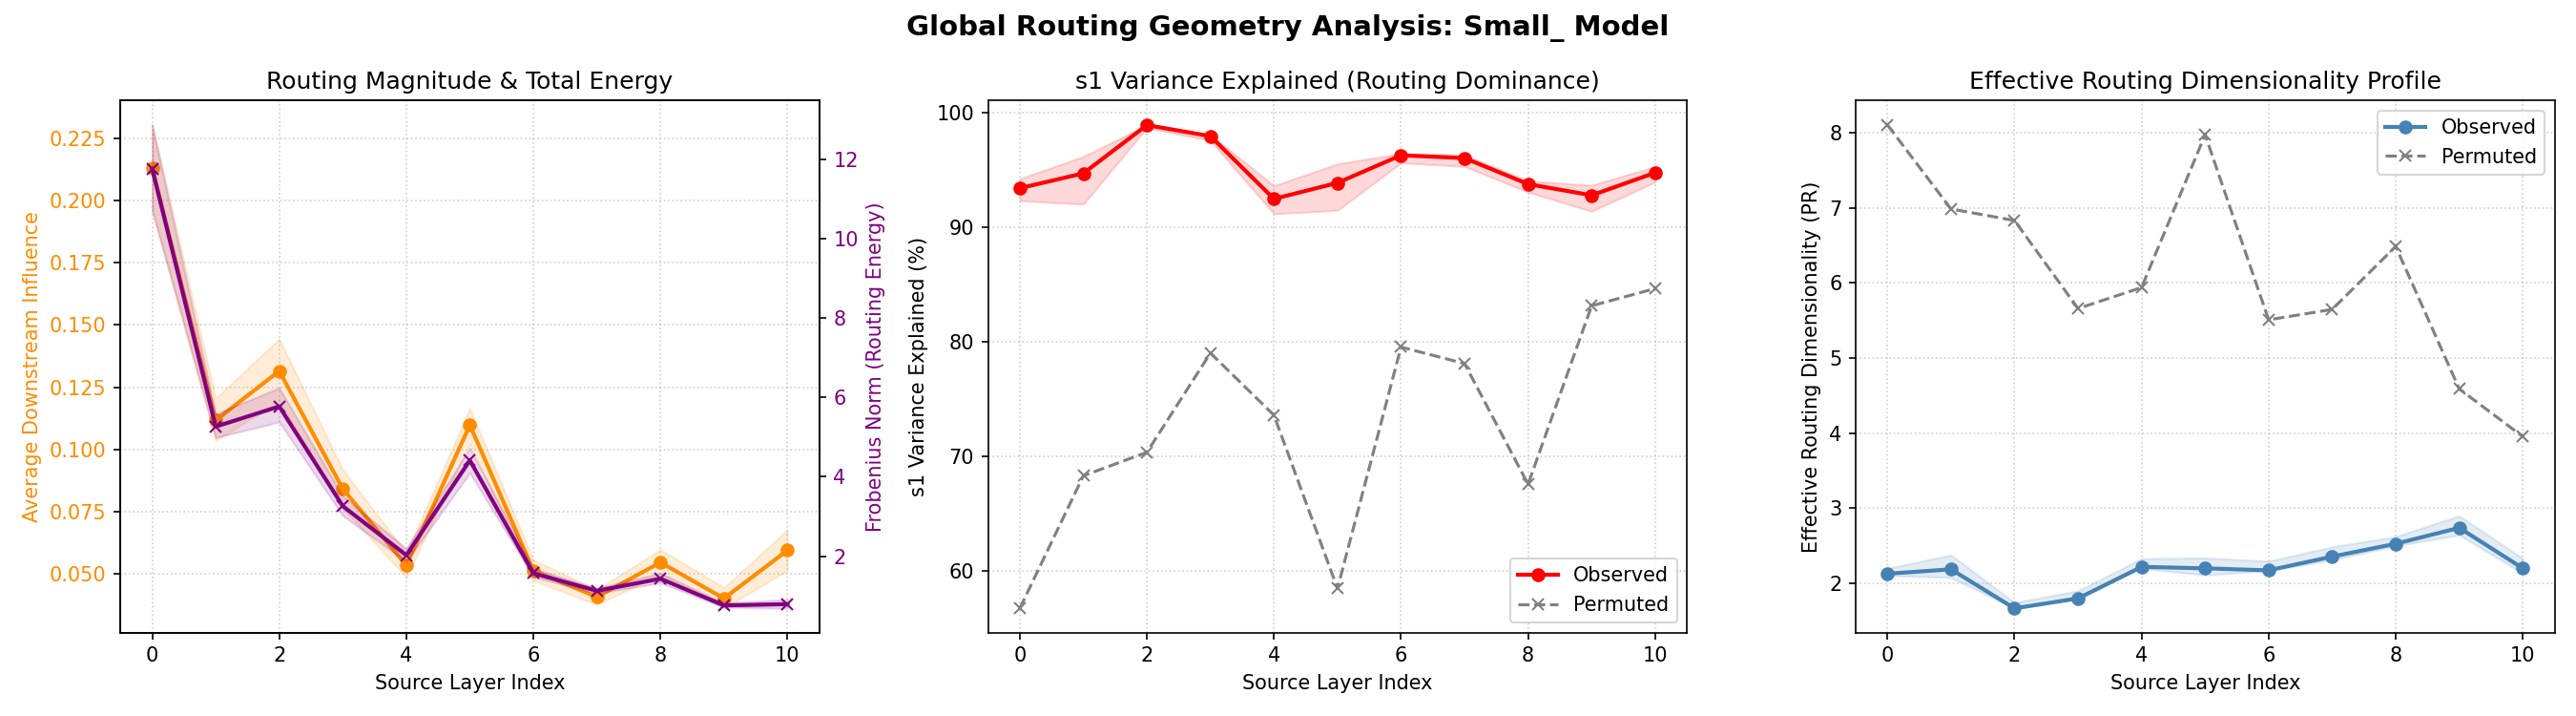
\includegraphics[width=\textwidth]{small_global_routing_geometry.png}
        \caption{GPT-2 Small Global Routing Profile}
        \label{fig:small_profile}
    \end{subfigure}
    \hfill
    \begin{subfigure}[b]{0.48\textwidth}
        \centering
        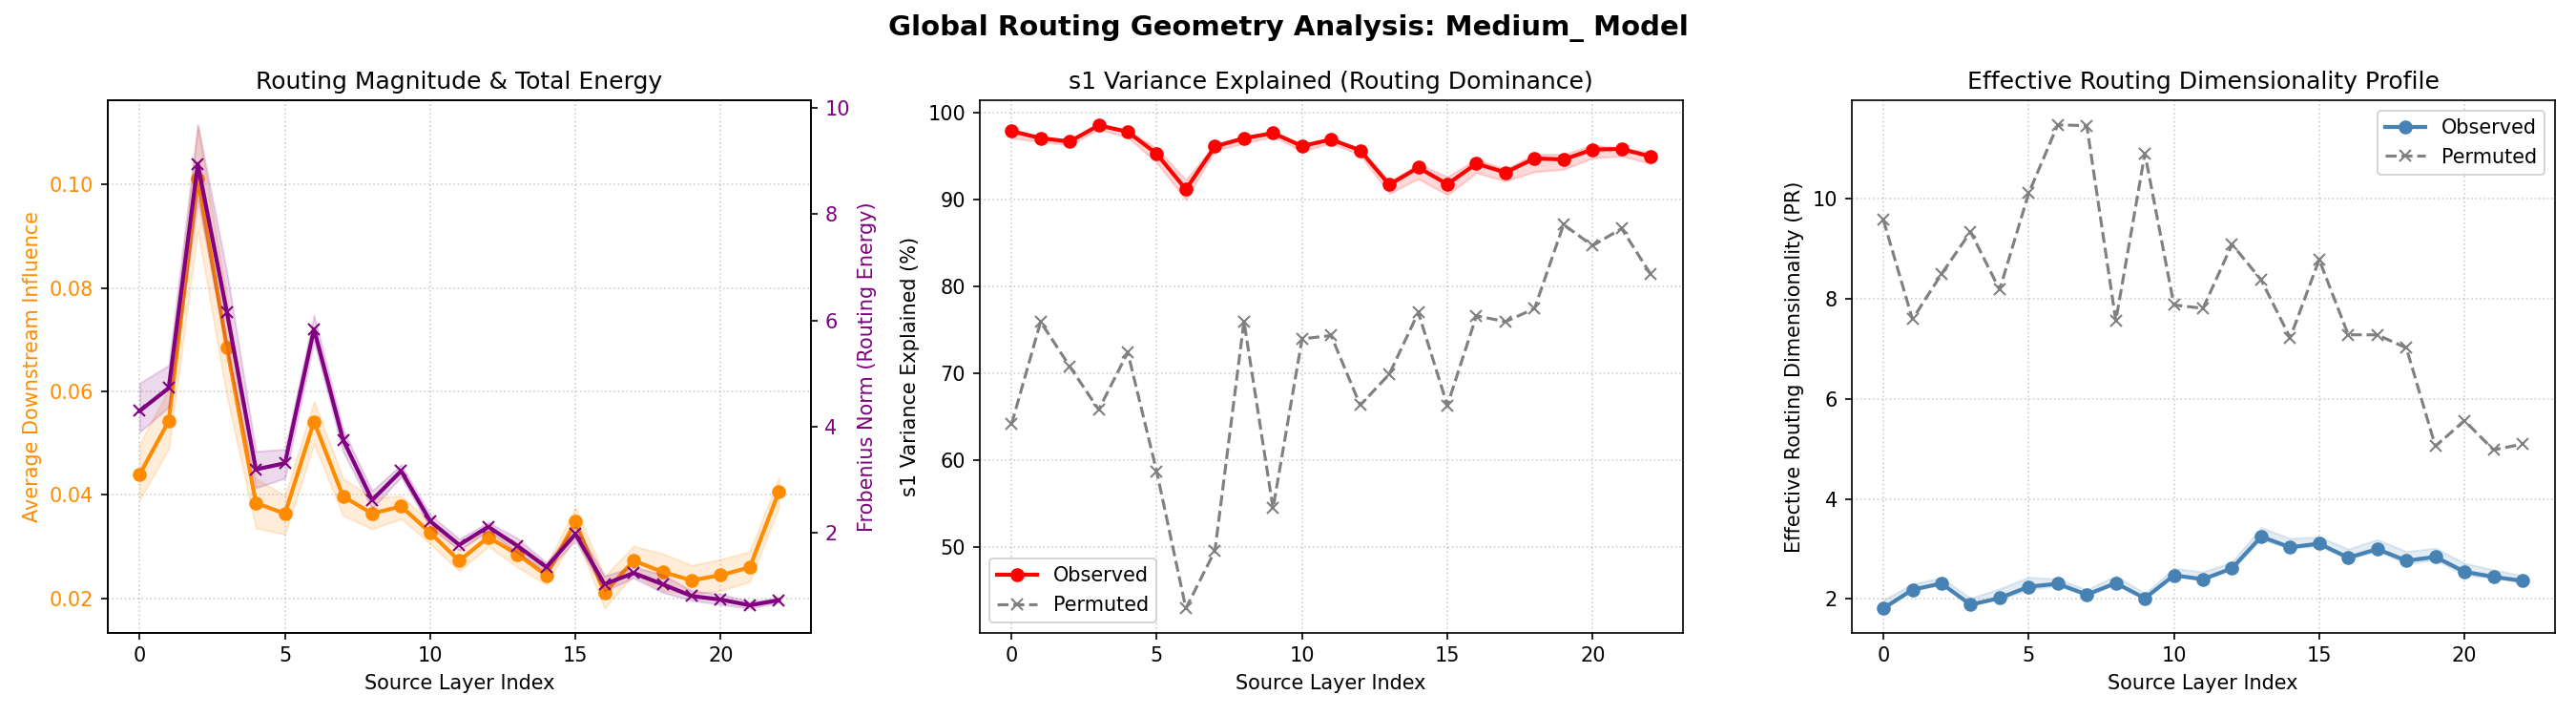
\includegraphics[width=\textwidth]{medium_global_routing_geometry.png}
        \caption{GPT-2 Medium Global Routing Profile}
        \label{fig:medium_profile}
    \end{subfigure}
    \\ \vspace{1em}
    \begin{subfigure}[b]{0.48\textwidth}
        \centering
        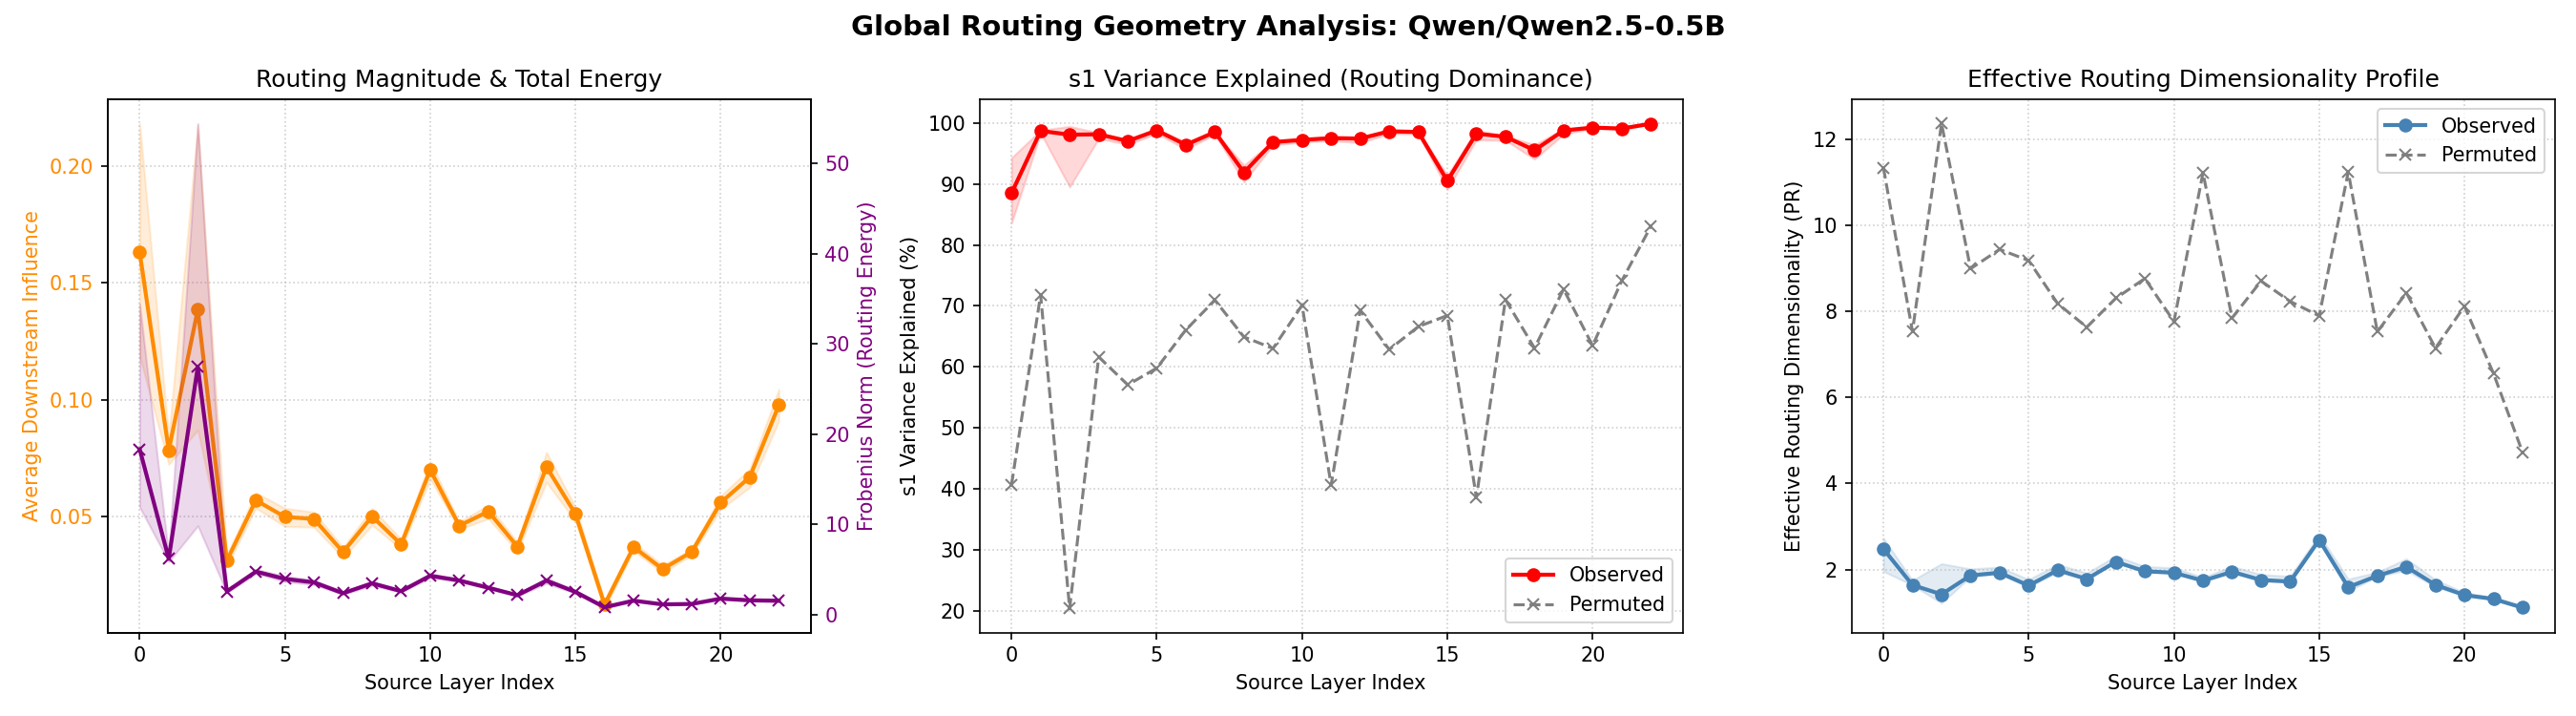
\includegraphics[width=\textwidth]{qwen_qwen2.5_0.5b_global_routing_geometry.png}
        \caption{Qwen2.5-0.5B Global Routing Profile}
        \label{fig:qwen_profile}
    \end{subfigure}
    \hfill
    \begin{subfigure}[b]{0.48\textwidth}
        \centering
        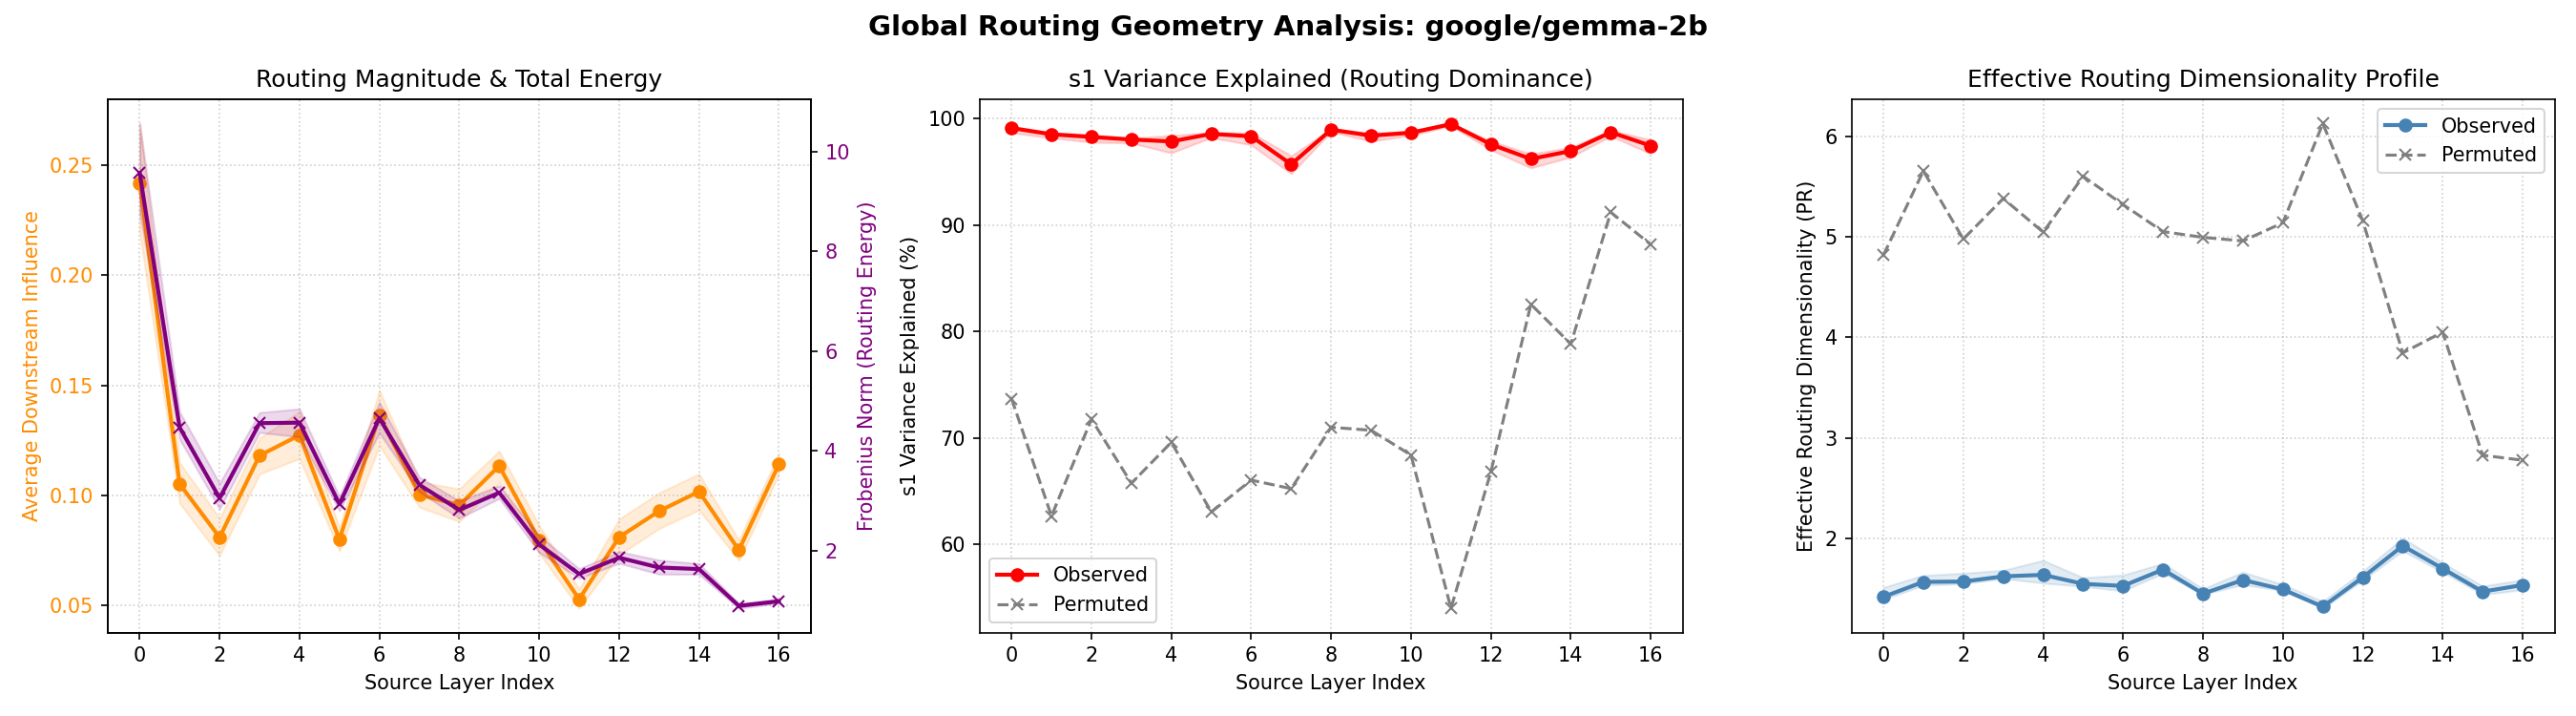
\includegraphics[width=\textwidth]{google_gemma_2b_global_routing_geometry.png}
        \caption{Gemma-2B Global Routing Profile}
        \label{fig:gemma_profile}
    \end{subfigure}
    \caption{Global routing profiles showing Frobenius norm, trace-based PR, and $s_1$ variance explained across source layers. The consistently low PR and high variance explained demonstrate a persistent low-rank structure across all models.}
    \label{fig:global_profiles}
\end{figure}

\subsection{Finding A: Highly Aligned Perturbation Direction}
To test if different layers project perturbations along a shared direction, we compute the cosine similarity between the first right singular vectors ($v_1$) of the influence matrices for every pair of source layers (excluding the diagonal self-comparisons).
\begin{itemize}[leftmargin=*]
    \item \textbf{GPT-2 Small Average Alignment:} \textbf{0.9756} (IQR: $[0.9634, 0.9912]$, Min: $0.9168$, Max: $0.9995$).
    \item \textbf{GPT-2 Medium Average Alignment:} \textbf{0.9758} (IQR: $[0.9682, 0.9924]$, Min: $0.8679$, Max: $0.9997$).
    \item \textbf{Pythia-70M Average Alignment:} \textbf{0.9506}.
    \item \textbf{Qwen2.5-0.5B Average Alignment:} \textbf{0.9359} (IQR: $[0.9507, 0.9886]$, Min: $0.5018$, Max: $0.9978$).
    \item \textbf{Gemma-2B Average Alignment:} \textbf{0.9617} (IQR: $[0.9524, 0.9786]$, Min: $0.8869$, Max: $0.9956$).
\end{itemize}
These results indicate that the shared perturbation direction generalizes across distinct decoder-only architectures. Downstream perturbations are highly aligned to a common principal axis that is nearly invariant across all layers.

\subsubsection{Statistical Significance: Isotropic Null Baseline}
To establish the statistical significance of these alignments, we perform a Monte Carlo simulation (10,000 trials) under a null hypothesis where the principal perturbation direction of each layer is isotropic and unaligned. Specifically, for each trial, we generate a pair of independent random unit vectors in the respective overlapping target dimensions for each layer pair. This constructs an empirical null distribution of the mean off-diagonal alignment.

Across all models, the observed alignments lie far outside the empirical null distribution. No simulated trial reached the observed alignment, yielding an empirical upper bound of $p < 1/10,001$. The empirical null 95\% confidence intervals (CIs) for isotropic alignments are:
\begin{itemize}[leftmargin=*]
    \item \textbf{Pythia-70M:} Observed: 0.9506 | Null 95\% CI: $[0.1288, 0.3328]$ ($p < 1/10,001$)
    \item \textbf{SmolLM-135M:} Observed: 0.9365 | Null 95\% CI: $[0.1012, 0.1186]$ ($p < 1/10,001$)
    \item \textbf{GPT-2 Small:} Observed: 0.9756 | Null 95\% CI: $[0.1112, 0.1682]$ ($p < 1/10,001$)
    \item \textbf{GPT-2 Medium:} Observed: 0.9758 | Null 95\% CI: $[0.0813, 0.0994]$ ($p < 1/10,001$)
    \item \textbf{Qwen2.5-0.5B:} Observed: 0.9359 | Null 95\% CI: $[0.0869, 0.1065]$ ($p < 1/10,001$)
    \item \textbf{Gemma-2B:} Observed: 0.9617 | Null 95\% CI: $[0.1260, 0.1640]$ ($p < 1/10,001$)
\end{itemize}

\begin{figure}[H]
    \centering
    \begin{subfigure}[b]{0.48\textwidth}
        \centering
        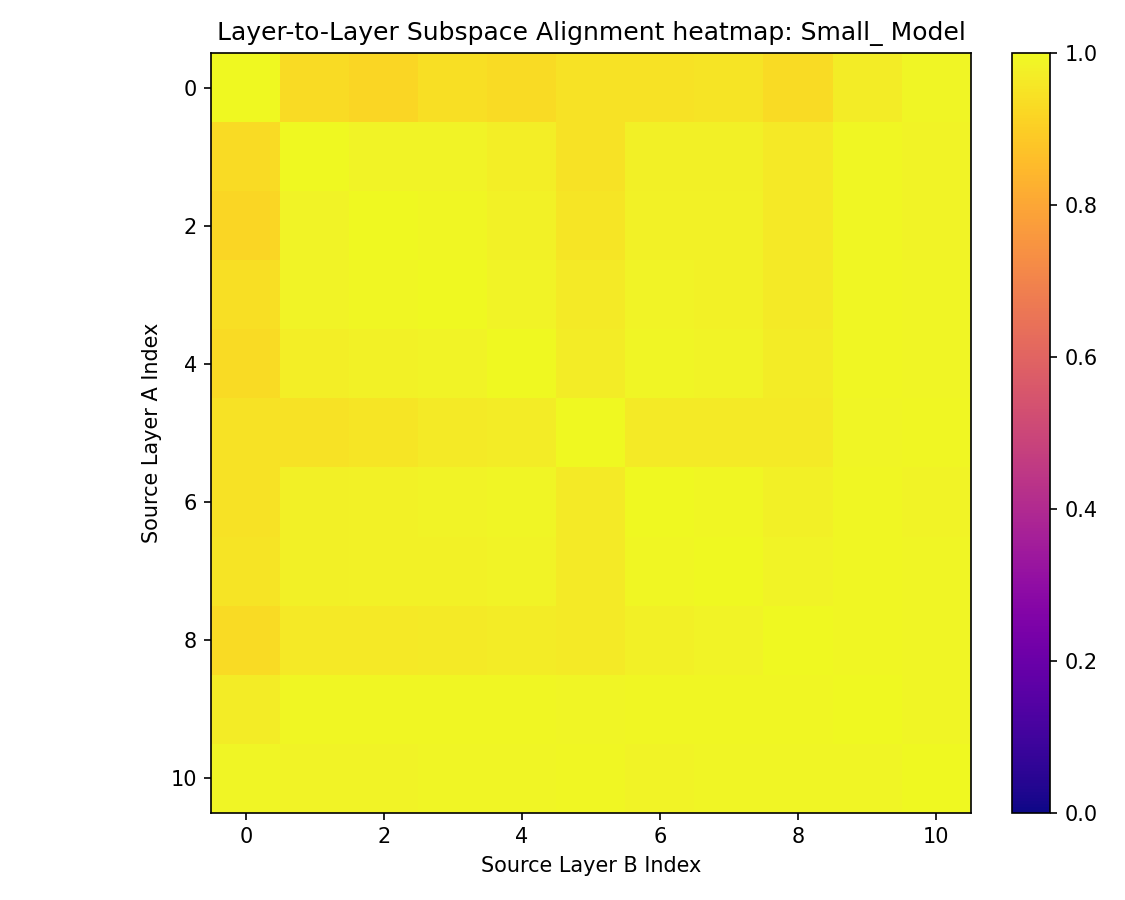
\includegraphics[width=\textwidth]{small_subspace_alignment_matrix.png}
        \caption{GPT-2 Small Subspace Alignment}
        \label{fig:small_align}
    \end{subfigure}
    \hfill
    \begin{subfigure}[b]{0.48\textwidth}
        \centering
        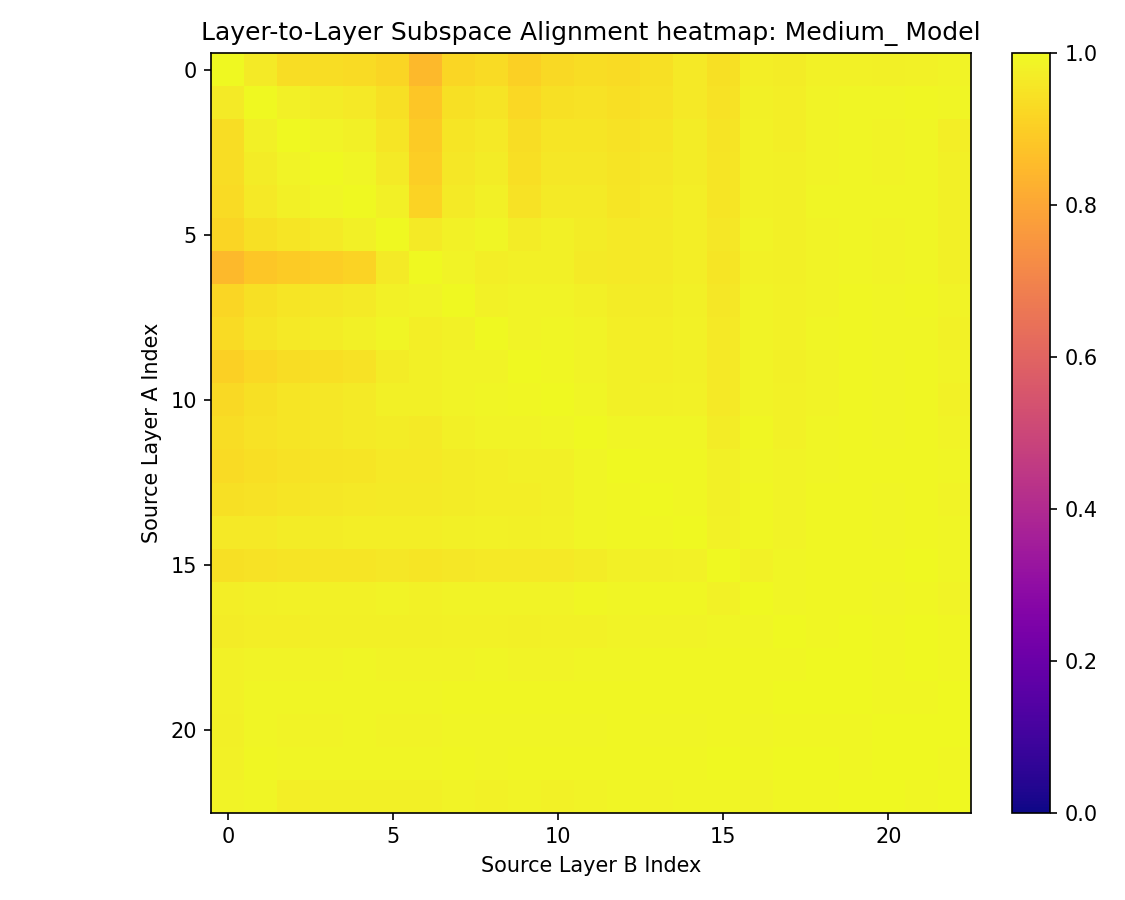
\includegraphics[width=\textwidth]{medium_subspace_alignment_matrix.png}
        \caption{GPT-2 Medium Subspace Alignment}
        \label{fig:medium_align}
    \end{subfigure}
    \\ \vspace{1em}
    \begin{subfigure}[b]{0.48\textwidth}
        \centering
        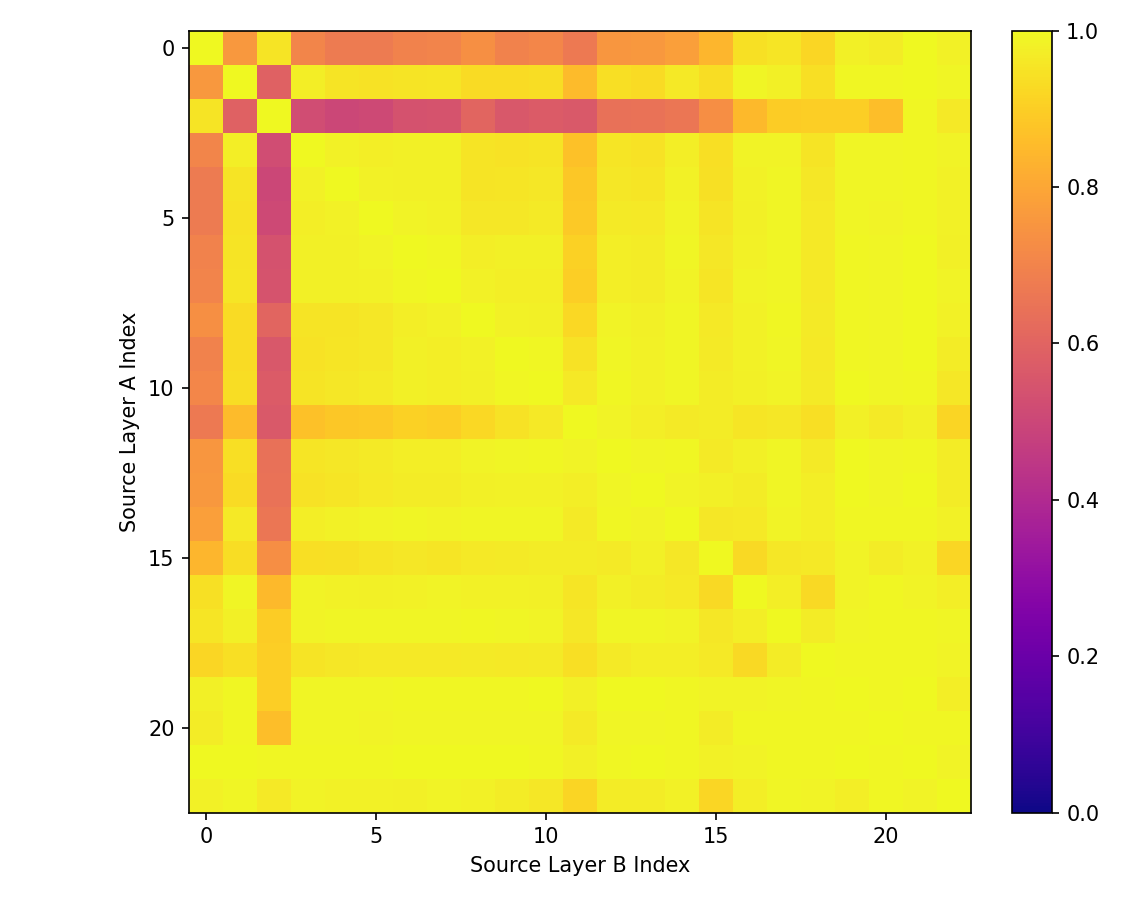
\includegraphics[width=\textwidth]{qwen_qwen2.5_0.5b_subspace_alignment_matrix.png}
        \caption{Qwen2.5-0.5B Subspace Alignment}
        \label{fig:qwen_align}
    \end{subfigure}
    \hfill
    \begin{subfigure}[b]{0.48\textwidth}
        \centering
        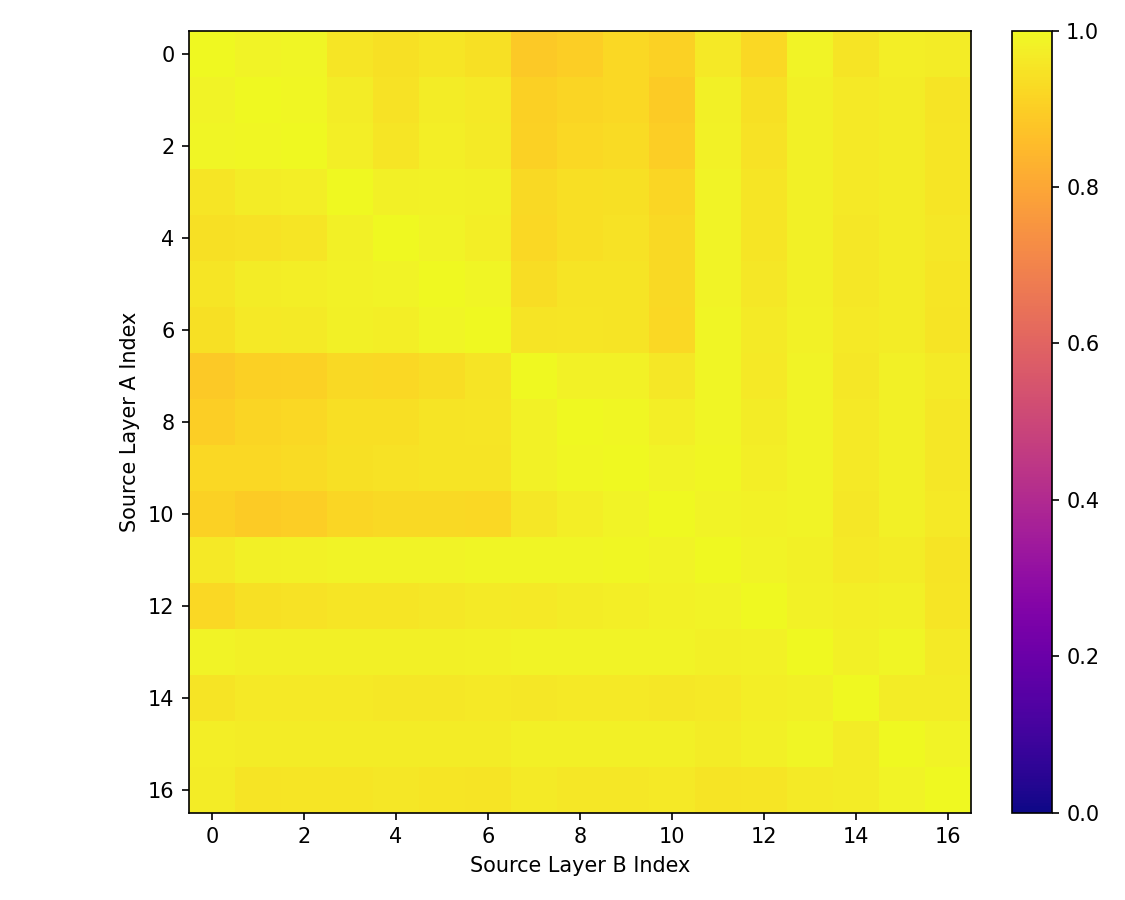
\includegraphics[width=\textwidth]{google_gemma_2b_subspace_alignment_matrix.png}
        \caption{Gemma-2B Subspace Alignment}
        \label{fig:gemma_align}
    \end{subfigure}
    \caption{Alignment matrices of the first right singular vector ($v_1$) across source layers, demonstrating consistently high off-diagonal similarity. This indicates that representation shifts from different source layers project along nearly identical dominant routing directions.}
    \label{fig:subspace_alignments}
\end{figure}

\subsection{Finding B: Subspace Metric Stability across Model Scales}
We analyze the relationship between the parameter scale of the model (ranging from 70M parameters to 2.5B parameters) and the shared routing properties. As shown in Figure~\ref{fig:scaling_analysis}, across the examined parameter range, the routing geometry metrics remain remarkably stable, providing evidence that the phenomenon is robust across model scale:
\begin{itemize}[leftmargin=*]
    \item \textbf{Subspace Alignment Stability:} The mean off-diagonal alignment stays tightly clustered between \textbf{0.93} and \textbf{0.98} across all tested parameter counts, remaining within a narrow range across the examined models.
    \item \textbf{Sparsity of Dimensionality:} The layer-wise average PR remains consistently low (typically \textbf{1.5 to 2.5}) across all six model scales, indicating that the low-dimensional constraint is a robust empirical property that is preserved even as model capacity and depth increase.
\end{itemize}

\begin{figure}[H]
    \centering
    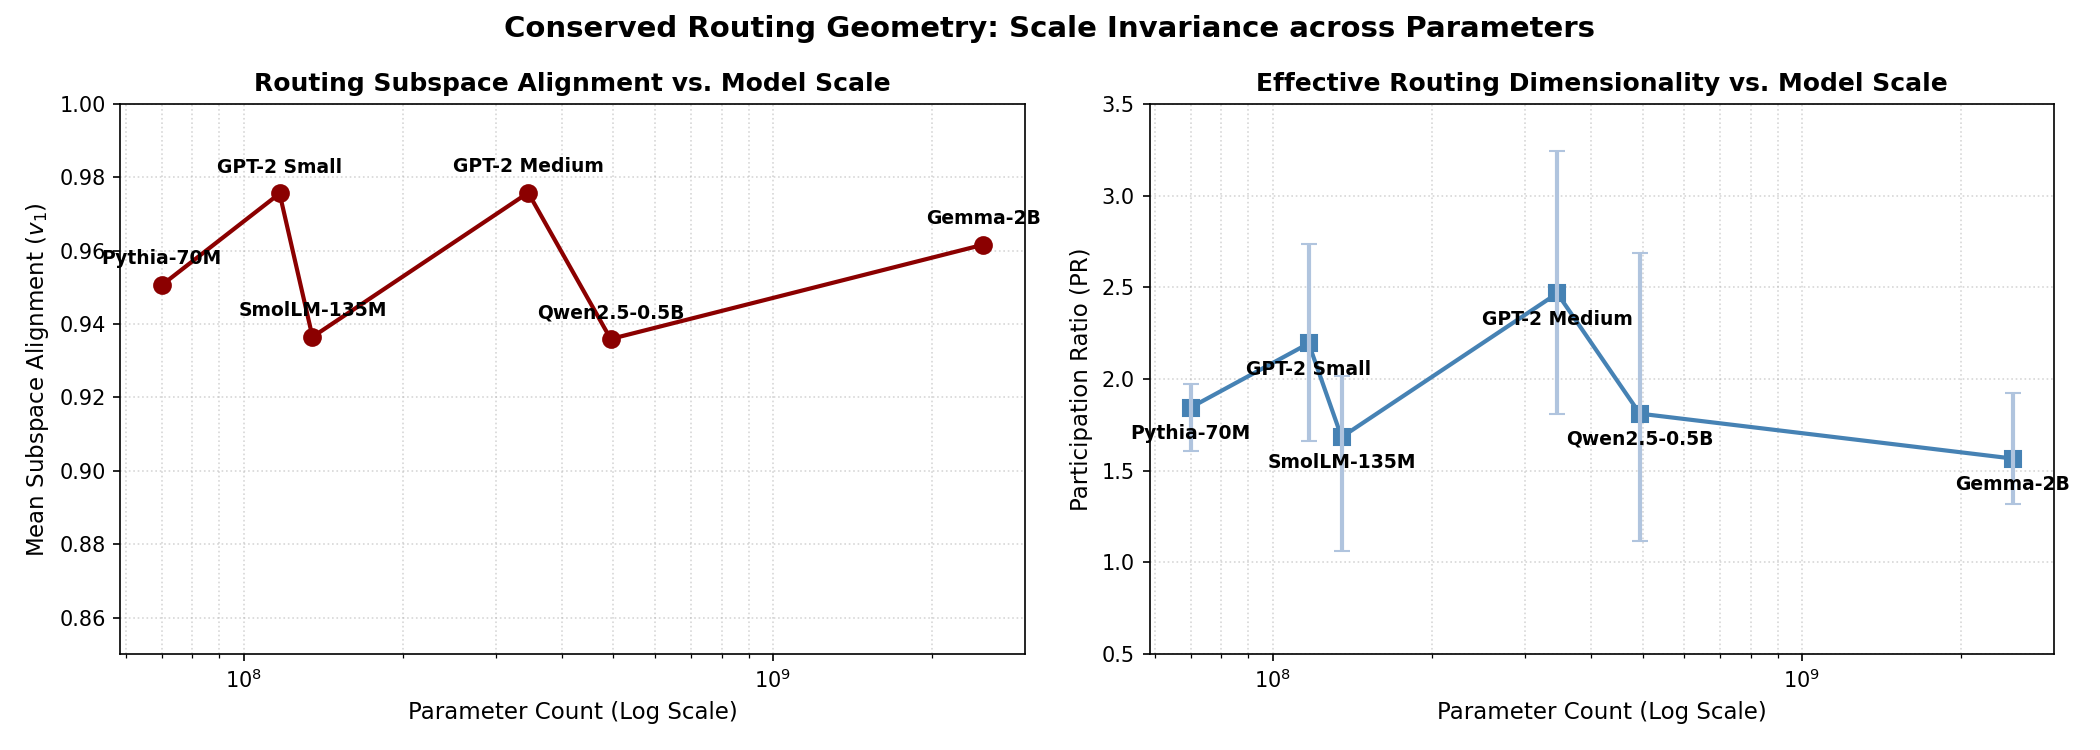
\includegraphics[width=0.85\textwidth]{scaling_analysis.png}
    \caption{Shared routing geometry metrics vs. model parameter scale. Left: Mean off-diagonal subspace alignment ($v_1$) is stable between 0.93 and 0.98. Right: Mean Participation Ratio (PR) remains low (1.5--2.5) across all model sizes (error bars denote min/max layer-wise PR range), showing strong scale robustness.}
    \label{fig:scaling_analysis}
\end{figure}

\subsection{Finding C: Low-Dimensional Subspace Collapse}
Across all models, the effective routing dimensionality (PR) remains consistently low and stable throughout the depth of the network, typically ranging between \textbf{1.0 and 3.2}. 
\begin{itemize}[leftmargin=*]
    \item In all cases, the observed PR is highly statistically distinct from the shuffled baseline controls. For example, at the Qwen2.5-0.5B peak (Layer 2), the observed PR of \textbf{1.42} represents an \textbf{81.2\%} reduction compared to the shuffled control baseline of \textbf{7.55}. For Gemma-2B, the observed PR of \textbf{1.42} (at Layer 00) represents a \textbf{70.5\%} reduction compared to the shuffled control of \textbf{4.82}.
    \item The first singular component is highly dominant across all layers, explaining \textbf{87.5\% to 99.9\%} of the downstream variance. At the Gemma-2B peak (Layer 00), the observed $s_1$ variance of \textbf{99.1\%} represents a \textbf{+25.4 percentage point increase} over the shuffled baseline (\textbf{73.7\%}).
    \item \textbf{Implication:} The observed low-rank structure is not a local anomaly but a globally shared property of representation routing.
\end{itemize}

\subsection{Finding D: Bridge/Peak Layers as Localized Amplitude Injectors}
While perturbation geometry ($v_1$ direction and low-dimensional collapse) is highly aligned across layers, the \emph{amplitude} and \emph{norm} of the perturbations show sharp, localized peaks at specific layers:
\begin{itemize}[leftmargin=*]
    \item \textbf{GPT-2 Small:} Layer 00 serves as the primary routing amplifier, exhibiting a global peak in Frobenius Routing Norm (\textbf{11.754}).
    \item \textbf{GPT-2 Medium:} Layer 02 acts as the primary amplifier, exhibiting a sharp global peak in Frobenius Routing Norm (\textbf{8.944}).
    \item \textbf{Qwen2.5-0.5B:} Layer 02 concentrates a massive Frobenius Routing Norm of \textbf{27.439}, which is \textbf{4.4x} higher than at Layer 01 and \textbf{18.0x} higher than at Layer 22.
    \item \textbf{Gemma-2B:} Layer 00 acts as the primary routing amplifier, exhibiting a global peak in Frobenius Routing Norm (\textbf{9.564}) and a Mean Influence of \textbf{0.2418}.
\end{itemize}

\textbf{Implication for Shared Routing:} These results demonstrate that the invariant object is not a specific, fixed bridge layer index across models. Instead, each architecture contains one or more early routing amplification layers whose precise depth varies (e.g., Layer 0 in GPT-2 Small and Gemma-2B vs. Layer 2 in GPT-2 Medium and Qwen2.5-0.5B). These layers act as localized amplitude injectors that drive large-amplitude perturbations directly into a globally aligned, shared low-dimensional routing manifold.

\subsection{Functional Relevance of the Shared Subspace}
To validate whether the dominant routing directions identified by SVD are functionally relevant, we perform three targeted intervention experiments on EleutherAI Pythia-70M using 15 prompts spanning code, mathematics, and natural language. We note that these functional intervention experiments were performed on Pythia-70M as an initial validation; extending them across additional model families is left for future work.

\textbf{Intervention design.} For each source layer $l$, the SVD of the influence matrix $\mathbf{I}^{(l)}$ yields left singular vectors $u_k^{(l)} \in \mathbb{R}^{H}$, where $H$ is the number of attention heads. To intervene on the model's hidden representations ($\mathbb{R}^{d_{\mathrm{model}}}$), we lift each head-coefficient vector into the full hidden space by replicating each head's scalar coefficient across its $d_h$-dimensional subspace and normalizing to unit norm. The resulting projection selectively removes variance along one geometric direction in head-coefficient space while preserving the remaining representation, avoiding the injection of out-of-distribution noise or arbitrary zeroing artifacts. We apply the intervention $x' = x - \alpha \operatorname{proj}_V(x)$ to the attention output projection and measure the resulting KL divergence of next-token predictions relative to the unperturbed model.

\textbf{Layer selection.} We intervene on layers 0--4 because our earlier routing analysis identified these as the layers exhibiting the highest Frobenius routing norm and strongest downstream influence (see Finding D), motivating their selection for functional validation.

\begin{enumerate}
    \item \textbf{Experiment A: Per-Layer Projection.} We project out $u_1^{(l)}$ at \emph{one layer at a time} (not simultaneously) and compare against 30 independently sampled random orthogonal baselines. As shown in Table~\ref{tab:per_layer_projection}, layers 0, 2, and 3 show statistically significant per-layer effects (Wilcoxon signed-rank $p < 0.05$), with Layer 0 ($1.17\times$, $p=0.013$) and Layer 3 ($1.19\times$, $p=0.018$) exhibiting the strongest isolated effects. Notably, the per-layer effects are heterogeneous: layers 1 and 4 do not show significant effects in isolation, suggesting that not every layer contributes equally to the routing subspace's functional role.

    \item \textbf{Experiment B: SVD Component Comparison.} To test whether the first singular direction exhibits the most consistent functional effect among the tested components, we compare multi-layer projections using $u_1$ vs. $u_2$, $u_3$, and $u_4$ across layers 0--4 simultaneously. As shown in Table~\ref{tab:svd_component_comparison}, $u_1$ produces the highest KL divergence ($0.060 \pm 0.004$) and is significantly larger than $u_2$ ($0.053 \pm 0.002$; Wilcoxon $p = 0.009$). However, $u_3$ produces a KL divergence ($0.059 \pm 0.004$) that is not significantly different from $u_1$ ($p = 0.300$), suggesting that functional importance is not perfectly predicted by singular value magnitude alone. This indicates that the first few singular directions may all encode meaningful routing structure, although $u_1$ remains the most consistently important across layers.

    \item \textbf{Experiment C: Multi-Layer Simultaneous Projection.} We project out $u_1^{(l)}$ at \emph{all layers 0--4 simultaneously} and sweep $\alpha \in [0.1, 1.0]$. As shown in Table~\ref{tab:multi_layer_projection}, the cumulative effect grows monotonically with $\alpha$, reaching $1.20\times$ at $\alpha = 1.0$ (Wilcoxon $p = 0.015$), consistent with the multi-layer intervention compounding across layers.

    \item \textbf{Node Redundancy vs. Specialization:} We rank downstream attention heads by their contribution (weight) in the dominant right singular vector $v_1$ of the influence matrix. We then compare the impact of ablating the top-$K$ heads (which participate heavily in the shared routing manifold) vs. the bottom-$K$ heads (which reside outside of it). As shown in Figure~\ref{fig:functional_node_importance}, ablating the bottom-$K$ heads causes a catastrophic degradation in prediction quality (e.g., at $K=4$, Bottom-$K$ KL = $0.260 \pm 0.009$ vs. Top-$K$ KL = $0.093 \pm 0.006$, a $2.8\times$ increase). These results are consistent with the hypothesis that heads with larger contributions to the shared routing subspace participate in more distributed, redundant computations, whereas heads with smaller contributions may support more specialized, non-redundant computations whose removal cannot be compensated for by the shared highway.
\end{enumerate}

% Table: Per-Layer Projection (Experiment A)
\begin{table}[H]
\centering
\caption{Per-layer projection at $\alpha = 1.0$: KL divergence when projecting out $u_1$ at one layer at a time vs. 30 random orthogonal baselines. Values are mean $\pm$ SE across 15 prompts. $p$-values from paired Wilcoxon signed-rank test.}
\label{tab:per_layer_projection}
\begin{tabular}{lcccc}
\toprule
\textbf{Layer} & \textbf{KL ($u_1$)} & \textbf{KL ($u_{\text{orth}}$, 30 avg)} & \textbf{Ratio} & \textbf{$p$ (Wilcoxon)} \\
\midrule
0 & 0.0519 $\pm$ 0.0036 & 0.0442 $\pm$ 0.0025 & 1.17x & 0.013 \\
1 & 0.0386 $\pm$ 0.0034 & 0.0391 $\pm$ 0.0027 & 0.99x & 0.661 \\
2 & 0.0413 $\pm$ 0.0040 & 0.0380 $\pm$ 0.0028 & 1.09x & 0.037 \\
3 & 0.0363 $\pm$ 0.0035 & 0.0305 $\pm$ 0.0026 & 1.19x & 0.018 \\
4 & 0.0164 $\pm$ 0.0022 & 0.0156 $\pm$ 0.0016 & 1.05x & 0.227 \\
\bottomrule
\end{tabular}
\end{table}

% Table: SVD Component Comparison (Experiment B)
\begin{table}[H]
\centering
\caption{SVD component comparison: KL divergence when projecting out $u_k$ (multi-layer, $\alpha = 1.0$). $p$-values test whether $u_1$ causes significantly greater KL than each alternative (paired Wilcoxon signed-rank, one-sided).}
\label{tab:svd_component_comparison}
\begin{tabular}{lcc}
\toprule
\textbf{Component} & \textbf{KL (mean $\pm$ SE)} & \textbf{$p$ vs. $u_1$ (Wilcoxon)} \\
\midrule
$u_1$ & 0.0603 $\pm$ 0.0042 & (reference) \\
$u_2$ & 0.0529 $\pm$ 0.0025 & 0.009 \\
$u_3$ & 0.0586 $\pm$ 0.0039 & 0.300 \\
$u_4$ & 0.0546 $\pm$ 0.0038 & 0.068 \\
\bottomrule
\end{tabular}
\end{table}

% Table: Multi-Layer Simultaneous Projection (Experiment C)
\begin{table}[H]
\centering
\caption{Multi-layer simultaneous projection (layers 0--4): KL divergence when projecting out $u_1$ at all layers simultaneously vs. 30 random orthogonal baselines across scaling factors $\alpha$. Values are mean $\pm$ SE across 15 prompts.}
\label{tab:multi_layer_projection}
\begin{tabular}{lcccc}
\toprule
\textbf{Scale ($\alpha$)} & \textbf{KL ($u_1$)} & \textbf{KL ($u_{\text{orth}}$, 30 avg)} & \textbf{Ratio} & \textbf{$p$ (Wilcoxon)} \\
\midrule
0.10 & 0.0294 $\pm$ 0.0028 & 0.0291 $\pm$ 0.0027 & 1.01x & 0.381 \\
0.30 & 0.0408 $\pm$ 0.0036 & 0.0360 $\pm$ 0.0027 & 1.13x & 0.047 \\
0.50 & 0.0453 $\pm$ 0.0040 & 0.0407 $\pm$ 0.0028 & 1.11x & 0.126 \\
0.70 & 0.0514 $\pm$ 0.0042 & 0.0450 $\pm$ 0.0027 & 1.14x & 0.060 \\
1.00 & 0.0603 $\pm$ 0.0042 & 0.0504 $\pm$ 0.0027 & 1.20x & 0.015 \\
\bottomrule
\end{tabular}
\end{table}

\begin{figure}[H]
    \centering
    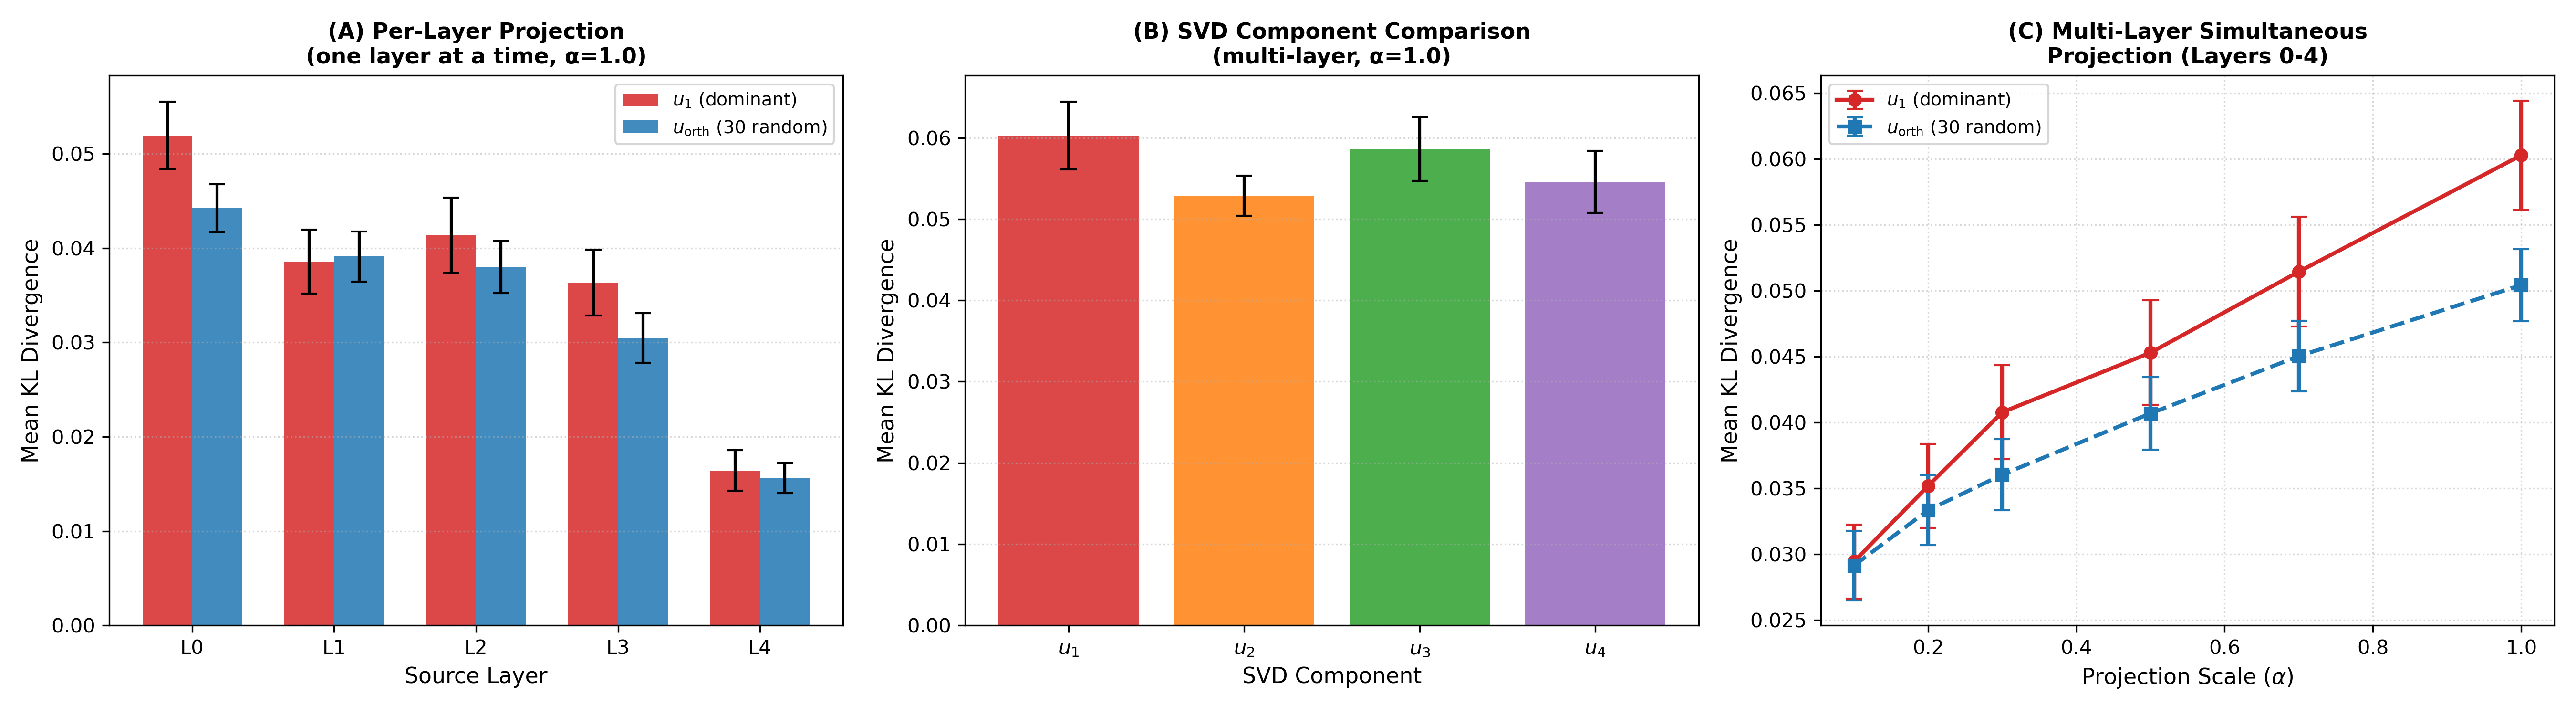
\includegraphics[width=\textwidth]{subspace_projection_comprehensive.png}
    \caption{Comprehensive functional validation of the routing subspace in Pythia-70M. (A) Per-layer projection: projecting out $u_1$ at individual layers shows significant effects at layers 0, 2, and 3. (B) SVD component comparison: $u_1$ produces the highest KL divergence, significantly exceeding $u_2$ ($p = 0.009$). (C) Multi-layer simultaneous projection: the cumulative effect grows monotonically with $\alpha$, reaching $1.20\times$ at $\alpha = 1.0$ ($p = 0.015$).}
    \label{fig:subspace_projection_comprehensive}
\end{figure}

\begin{figure}[H]
    \centering
    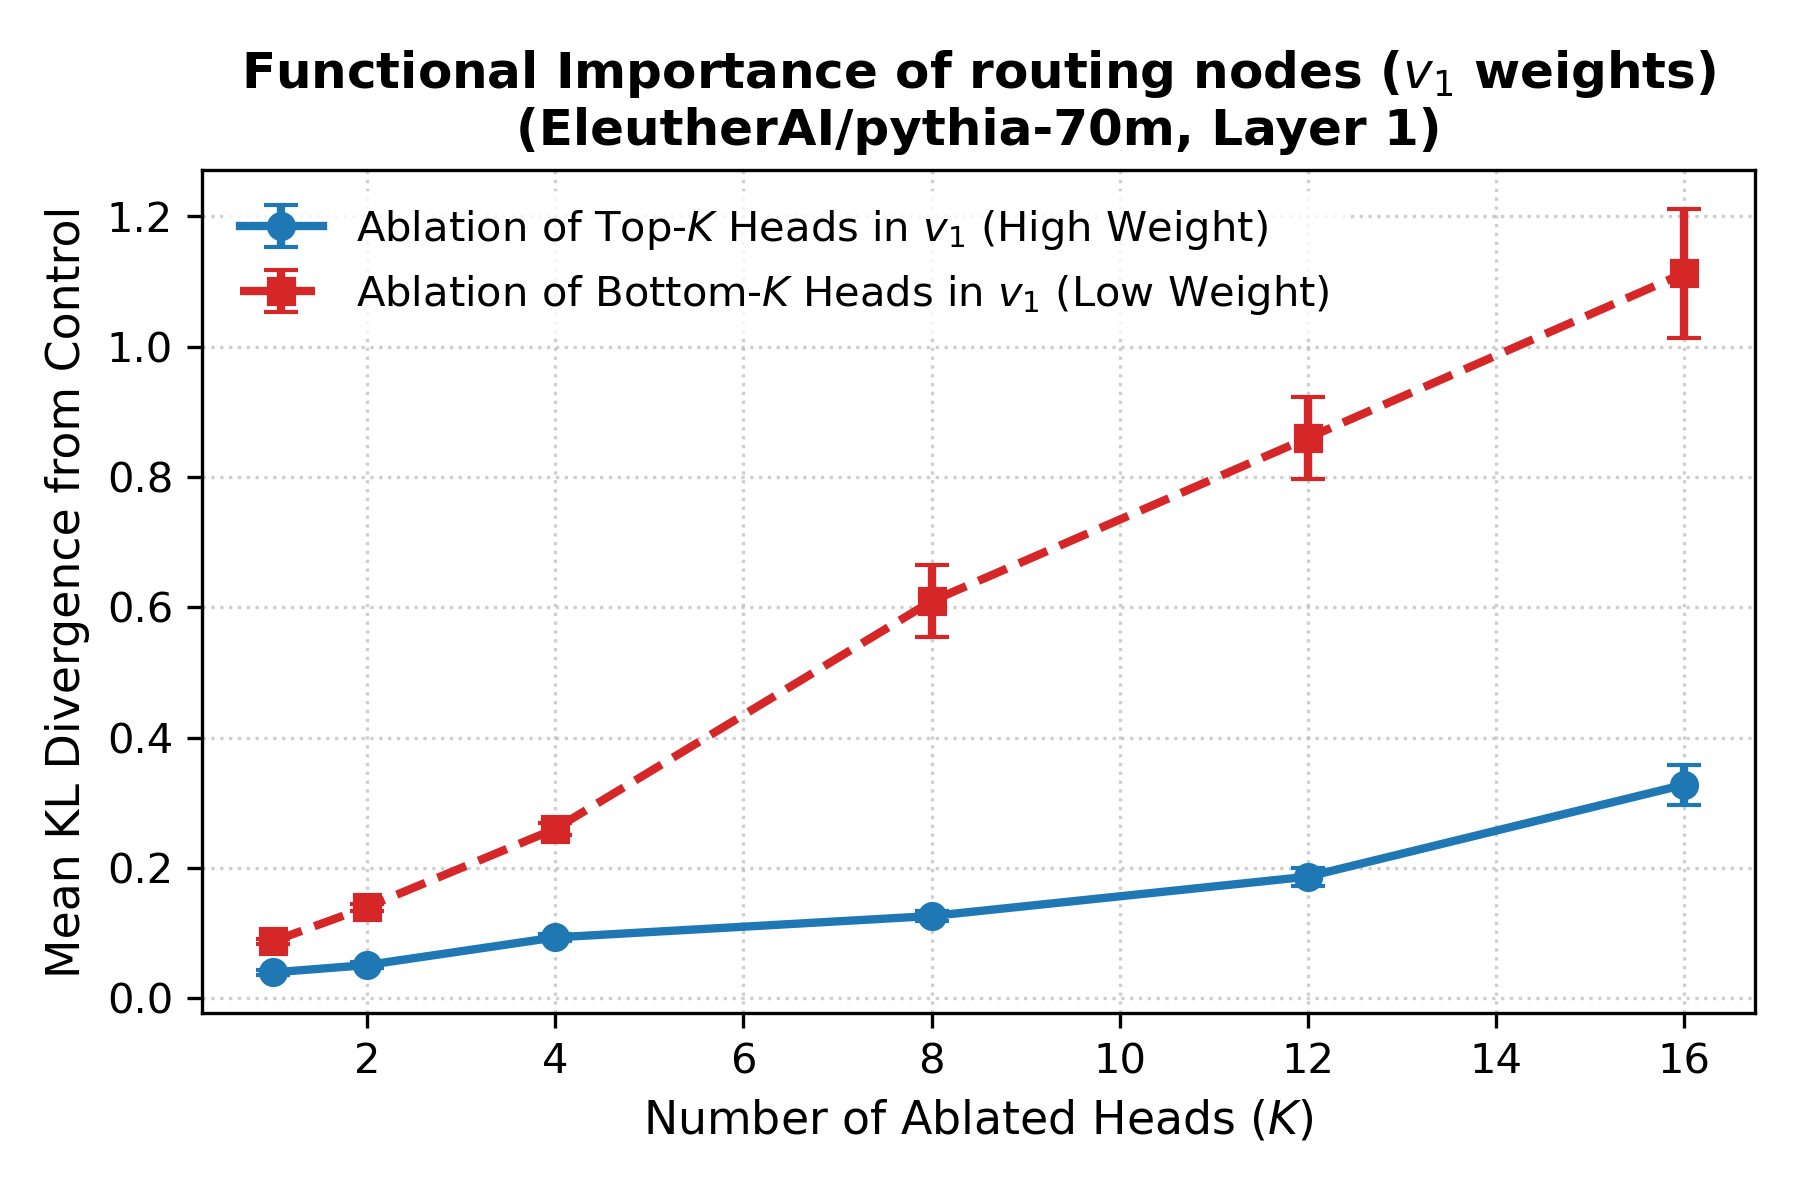
\includegraphics[width=0.65\textwidth]{functional_node_importance.png}
    \caption{Functional importance of routing nodes in Pythia-70M. Ablating the bottom-$K$ heads in $v_1$ (which operate outside the shared routing subspace) causes a catastrophic increase in KL divergence compared to the top-$K$ heads, consistent with the hypothesis that the shared subspace functions as a robust, redundant routing highway while heads outside it support more specialized computations.}
    \label{fig:functional_node_importance}
\end{figure}

% ═════════════════════════════════════════════════════════════════════════════
\section{Discussion and Visualization}
\label{sec:discussion}

The discovery of a globally aligned, low-dimensional routing geometry has significant implications for both network science and practical pruning algorithms:
\begin{enumerate}
    \item \textbf{Reframing Circuits:} Instead of independent, graph-like attention circuits, representations flow through a highly constrained, shared coordinate system.
    \item \textbf{Flood Pruning Implications:} Rather than pruning based on localized metrics, pruning algorithms should preserve the overall energy and alignment of the shared subspace, preventing the removal of localized high-amplitude injectors like bridge heads.
\end{enumerate}

We emphasize that our observations are empirical rather than mechanistic and do not by themselves establish the causal origin of the shared routing geometry. Crucially, however, the existence of a globally aligned routing manifold does not contradict the presence of localized, task-specific circuits (e.g., induction circuits or indirect object identification circuits). Instead, it suggests that while individual attention heads perform distinct computations, the resulting downstream updates are projected into a common, low-dimensional coordinate system. Under this view, the shared routing geometry serves as the shared communication highway, while local circuits act as specialized transmitters and receivers that inject signals into this highway. By framing representation routing as a low-dimensional manifold, our framework complements circuit discovery, offering a unified subspace perspective that simplifies how disparate circuits interact and propagate their outputs downstream.

\textbf{Functional validation nuances.} The projection intervention experiments (Section~\ref{sec:results}) reveal that the functional importance of singular directions does not perfectly mirror their spectral ranking. While $u_1$ produces the most consistent effect and is significantly more impactful than $u_2$, the third singular direction $u_3$ produces a surprisingly comparable KL divergence despite explaining less than 0.5\% of the singular-value variance. One possible interpretation is that the first few singular directions all encode functionally meaningful routing structure---for example, distinct routing channels that serve different computational roles---while only the first direction captures the dominant, shared routing highway. Investigating whether this pattern replicates across other architectures is an important direction for future work. We also note that while the projection effects are statistically significant (Wilcoxon $p < 0.05$), they are modest in absolute magnitude (ratios of 1.1--1.2$\times$), consistent with the expectation that removing one geometric direction from a distributed representation should produce a small but systematic perturbation rather than a catastrophic failure.

\section{Limitations and Future Work}
\label{sec:limitations}

While our findings of a shared routing geometry generalize across multiple transformer families, several limitations should be noted:
\begin{itemize}[leftmargin=*]
    \item \textbf{Model Families \& Architectural Scope:} Our empirical study is restricted to decoder-only autoregressive language models. While we evaluated models spanning different tokenizer vocabularies, routing configurations, and activation functions, we have not examined encoder-decoder architectures (e.g., T5) or encoder-only models (e.g., BERT), where routing constraints may differ due to bidirectional attention patterns.
    \item \textbf{Model Scale Boundaries:} The model scales evaluated in this study range from 70M to 2.5B parameters. Although the metrics remain remarkably stable across this range, providing evidence that the phenomenon is consistent across the examined parameter range, we have not tested massive, multi-billion or trillion-parameter frontier models where routing subspaces might show more complex multi-modal behavior.
    \item \textbf{Linear Subspace Focus:} Our analysis maps routing alignment using singular value decomposition (SVD) and cosine similarity of the first right singular vector ($v_1$), focusing on the dominant linear subspace. This approach does not capture potential non-linear interactions or routing channels that reside in the higher-order components.
    \item \textbf{Functional Validation Scope:} The functional intervention experiments were performed on Pythia-70M only. While the geometric findings replicate across six model families, the functional relevance results remain single-model evidence. Additionally, the effect sizes of the projection interventions are modest (1.1--1.2$\times$), and future work should assess whether these effects scale with model size or generalize to downstream task performance metrics beyond next-token KL divergence.
\end{itemize}

A natural next step is to expand this framework to extract the exact directed dependency networks from these influence matrices, performing community detection and bottleneck analysis to locate key articulation points in the network topology.

\bibliographystyle{abbrvnat}
\bibliography{references}

\end{document}
